\documentclass{article}

\usepackage[T1]{fontenc}
\usepackage{libertine}

\usepackage{fancyhdr}
\usepackage{extramarks}
\usepackage{amsmath}
\usepackage{amsthm}
\usepackage{amsfonts}
\usepackage{tikz}
\usepackage{algorithm}
\usepackage{algpseudocode}

\usetikzlibrary{automata,positioning}

%
% Basic Document Settings
%

\topmargin=-0.45in
\evensidemargin=0in
\oddsidemargin=0in
\textwidth=6.5in
\textheight=9.0in
\headsep=0.25in

\linespread{1.1}

\pagestyle{fancy}
\lhead{\hmwkAuthorName}
\chead{\hmwkClass: \hmwkTitle}
\rhead{\firstxmark}
\lfoot{\lastxmark}
\cfoot{\thepage}

\renewcommand\headrulewidth{0.4pt}
\renewcommand\footrulewidth{0.4pt}

\setlength\parindent{0pt}

%
% Create Problem Sections
%

\newcommand{\enterProblemHeader}[1]{
    \nobreak\extramarks{}{Problem \arabic{#1} continued on next page\ldots}\nobreak{}
    \nobreak\extramarks{Problem \arabic{#1} (continued)}{Problem \arabic{#1} continued on next page\ldots}\nobreak{}
}

\newcommand{\exitProblemHeader}[1]{
    \nobreak\extramarks{Problem \arabic{#1} (continued)}{Problem \arabic{#1} continued on next page\ldots}\nobreak{}
    \stepcounter{#1}
    \nobreak\extramarks{Problem \arabic{#1}}{}\nobreak{}
}

\setcounter{secnumdepth}{0}
\newcounter{partCounter}
\newcounter{homeworkProblemCounter}
\setcounter{homeworkProblemCounter}{1}
\nobreak\extramarks{Problem \arabic{homeworkProblemCounter}}{}\nobreak{}

%
% Homework Problem Environment
%
% This environment takes an optional argument. When given, it will adjust the
% problem counter. This is useful for when the problems given for your
% assignment aren't sequential. See the last 3 problems of this template for an
% example.
%
\newenvironment{homeworkProblem}[1][-1]{
    \ifnum#1>0
        \setcounter{homeworkProblemCounter}{#1}
    \fi
    \section{Problem \arabic{homeworkProblemCounter}}
    \setcounter{partCounter}{1}
    \enterProblemHeader{homeworkProblemCounter}
}{
    \exitProblemHeader{homeworkProblemCounter}
}

%
% Homework Details
%   - Title
%   - Due date
%   - Class
%   - Section/Time
%   - Instructor
%   - Author
%

\newcommand{\hmwkTitle}{Homework\ \#2}
\newcommand{\hmwkDueDate}{February 15, 2018}
\newcommand{\hmwkClass}{Design and Analysis of Algorithms}
\newcommand{\hmwkClassInstructor}{Professor Kasturi Varadarajan}
\newcommand{\hmwkAuthorName}{\textbf{Alic Szecsei}}

%
% Title Page
%

\title{
    \vspace{2in}
    \textmd{\textbf{\hmwkClass:\ \hmwkTitle}}\\
    \normalsize\vspace{0.1in}\small{Due\ in\ class\ on\ \hmwkDueDate}\\
    \vspace{0.1in}\large{\textit{\hmwkClassInstructor}}
    \vspace{3in}
}

\author{\hmwkAuthorName}
\date{}

\renewcommand{\part}[1]{\textbf{\large Part \Alph{partCounter}}\stepcounter{partCounter}\\}

%
% Various Helper Commands
%

% Useful for algorithms
\newcommand{\alg}[1]{\textsc{\bfseries \footnotesize #1}}

% For derivatives
\newcommand{\deriv}[1]{\frac{\mathrm{d}}{\mathrm{d}x} (#1)}

% For partial derivatives
\newcommand{\pderiv}[2]{\frac{\partial}{\partial #1} (#2)}

% Integral dx
\newcommand{\dx}{\mathrm{d}x}

% Alias for the Solution section header
\newcommand{\solution}{\textbf{\large Solution}}

% Probability commands: Expectation, Variance, Covariance, Bias
\newcommand{\E}{\mathrm{E}}
\newcommand{\Var}{\mathrm{Var}}
\newcommand{\Cov}{\mathrm{Cov}}
\newcommand{\Bias}{\mathrm{Bias}}

\begin{document}

\maketitle

\pagebreak

\begin{homeworkProblem}
Suppose we are given an array $A[1..n]$ with the special property that $A[1] \geq A[2]$ and $A[n-1] \leq A[n]$. We say that an element $A[x]$ is a \emph{local minimum} if it is less than or equal to both its neighbors, or more formally, if $A[x-1] \geq A[x]$ and $A[x] \leq A[x+1]$. For example, there are six local minima in the following array:\\
\begin{table}[h]
	\centering
	\begin{tabular}{ | *{15}{c |} c | }
		\hline
		9 & \textbf{7} & 7 & 2 & \textbf{1} & 3 & 7 & 5 & \textbf{4} & 7 & \textbf{3} & \textbf{3} & 4 & 8 & \textbf{6} & 9 \\
		\hline
\end{tabular}
	\caption{Example array}
	\label{tab:ExampleArray}
\end{table}


We can obviously find a local minimum in $O(n)$ time by scanning through the array. Describe and analyze an algorithm that finds a local minimum in $O(\log n)$ time. \emph{[Hint: With the given boundary conditions, the array \textbf{must} have at least one local minimum. Why?]}\\

\solution

\end{homeworkProblem}

\pagebreak

\begin{homeworkProblem}
Suppose we are given two sorted arrays $A[1..n]$ and $B[1..n]$ and an integer $k$. Describe an algorithm to find the $k$th smallest element in the union of $A$ and $B$ in $\Theta(\log n)$ time. For example, if $k = n$, your algorithm should return the smallest element of $A \cup B$; if $k = n$, your algorithm should return the median of $A \cup B$. You can assume that the arrays contain no duplicate elements. \emph{[Hint: First solve the special case $k = n$.]}\\

\solution


\end{homeworkProblem}

\pagebreak

\begin{homeworkProblem}
For this problem, a \emph{subtree} of a binary tree means any connected subgraph. A binary tree is \emph{complete} if every internal node has two children, and every leaf has exactly the same depth. Describe and analyze a recursive algorithm to compute the \emph{largest complete subtree} of a given binary tree. Your algorithm should return the root and the depth of this subtree.

\begin{figure}[h]
	\centering
		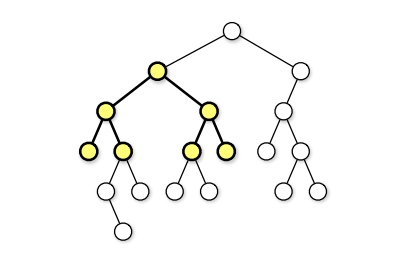
\includegraphics{images/binary-subtree.png}
	\caption{The largest complete subtree of this binary tree has depth 2.}
	\label{fig:binary-subtree}
\end{figure}

\solution



\end{homeworkProblem}

\pagebreak

\begin{homeworkProblem}
\begin{enumerate}
	\item Let $A[1..m]$ and $B[1..n]$ be two arbitrary arrays. A \emph{common subsequence} of $A$ and $B$ is both a subsequence of $A$ and a subsequence of $B$. Give a simple recursive definition for the function $lcs(A,B)$, which gives the length of the \emph{longest} common subsequence of $A$ and $B$.
	\item Call a sequence $X[1..n]$ \emph{oscillating} if $X[i] < X[i+1]$ for all even $i$, and $X[i] > X[i+1]$ for all odd $i$. Give a simple recursive definition for the function $los(A)$, which gives the length of the longest oscillating subsequence of an arbitrary array $A$ of integers.
	\item Call a sequence $X[1..n]$ \emph{accelerating} if $2 \times X[i] < X[i-1] + X[i+1]$ for all $i$. Give a simple recursive definition for the function $lxs(A)$, which gives the length of the longest accelerating subsequence of an arbitrary array $A$ of integers.
\end{enumerate}

\solution



\end{homeworkProblem}

\end{document}